\documentclass[11pt,a4paper]{article}

% --- Pakete ---
\usepackage[ngerman]{babel}
\usepackage[utf8]{inputenc}
\usepackage[T1]{fontenc}
\usepackage{lmodern}
\usepackage{geometry}
\usepackage{longtable}
\usepackage{float} 
\usepackage{float} 
\geometry{
  a4paper,
  left=2.5cm,
  right=2.5cm,
  top=2.5cm,
  bottom=2.5cm
}
\usepackage{setspace}
\setstretch{1.24}
\usepackage{microtype}
\usepackage{csquotes}
\usepackage{amsmath,amssymb}
\usepackage{graphicx}
\usepackage{caption}
\usepackage{subcaption}
\usepackage{siunitx}
\sisetup{detect-all}
\usepackage{booktabs}
\usepackage{hyperref}
\usepackage{fancyhdr}
\usepackage{mhchem}

% --- Kopf- und Fußzeile ---
\pagestyle{fancy}
\fancyhf{}
\fancyhead[L]{\nouppercase{\leftmark}}
\fancyfoot[C]{\thepage}
\renewcommand{\sectionmark}[1]{%
  \markboth{\thesection\ #1}{}%
}

% --- Nummerierte Gleichungen ---
\numberwithin{equation}{section}

% --- Abbildungs- und Tabellenbeschriftungen ---
\captionsetup{font=small,labelfont=bf}

% --- Metadaten ---
\newcommand{\Lehrveranstaltung}{Praktikum Physikalische Eigenschaften der Materialien}
\newcommand{\Universitaet}{Universität Augsburg}
\newcommand{\Semester}{Wintersemester 2025/2026}
\newcommand{\Versuchsnummer}{1}
\newcommand{\Versuchstitel}{Brennstoffzelle}
\newcommand{\Gruppe}{C}
\newcommand{\Versuchsdatum}{02.03.2026}
\newcommand{\Abgabedatum}{TT.MM.JJJJ}
\newcommand{\Abgabeart}{Gemeinsames Versuchsprotokoll}
\newcommand{\Autor}{Fabio Piskorz, Fabio Nogielsky, Konstantin Szantho von Radnoth}

% ---------------------------------------------------
% Titelseite
% ---------------------------------------------------
\begin{document}
\pagenumbering{gobble}

\begin{titlepage}
    \centering
    % --- Uni-Logo (Datei logo.png im gleichen Ordner ablegen) ---
  %  \includegraphics[width=0.35\textwidth]{logo.png}\par
    \vspace{1.0cm}
    {\Large \Lehrveranstaltung\par}
    \vspace{0.5cm}
    {\large \Universitaet\par}
    \vspace{0.5cm}
    {\large \Semester\par}
    \vspace{1.5cm}
    {\LARGE \Abgabeart\par}
    \vspace{0.5cm}
    {\Large Versuchsnummer: \Versuchsnummer\par}
    \vspace{0.5cm}
    {\Large Versuchstitel: \Versuchstitel\par}
    \vspace{1.5cm}
    {\large Gruppe \Gruppe\par}
    \vspace{0.5cm}
    {\large Autor(en): \Autor\par}
    \vspace{1.5cm}
    {\large Versuchsdatum: \Versuchsdatum\par}
    \vspace{0.5cm}
    {\large Abgabedatum: \Abgabedatum\par}
    \vfill
\end{titlepage}

% ab hier Seitenzahlen normal
\pagenumbering{arabic}

% ---------------------------------------------------
% 1 Einleitung
% ---------------------------------------------------
\section{Einleitung}

Brennstoffzellen stellen einen vielversprechenden Ansatz für eine klimaneutrale Energieversorgung dar, da sie Wasserstoff elektrochemisch in elektrische Energie umwandeln und lediglich Wasser sowie Wärme als Reaktionsprodukte erzeugen. Im Rahmen der Energiewende gewinnen sie durch ihre hohe gravimetrische Energiedichte und Emissionsfreiheit an technischer Relevanz. Der Versuch behandelt das Funktionsprinzip von PEM-Elektrolyseur und PEM-Brennstoffzelle als zentrale Komponenten eines Wasserstoff-Energiesystems. Mittels U-I-Kennlinienaufnahmen und Wirkungsgradbestimmungen werden die Effizienzen der Energiewandler sowie irreversible Verluste durch Aktivierungs-, Ohmsche- und Konzentrationsüberspannungen experimentell charakterisiert.

% ---------------------------------------------------
% 2 Theoretische Grundlagen
% ---------------------------------------------------
\section{Theoretische Grundlagen}

\subsection{PEM-Elektrolyseur}
Der Elektolyseur zerlegt durch elektrischen Strom Wasser ($H_{\text{2}}O$) in seine Bestandteile Wasserstoff ($H_{\text{2}}$) und Sauerstoff ($O_{\text{2}}$). Die dabei ablaufende Reaktion l\"asst sich mithilfe Reaktionsgleichung \ref{eq:ele} beschreiben.
\begin{align}
\ce{2H2O &-> 4H+ + 4e- + O2} \nonumber \\
\ce{4H+ + 4e- &-> 2H2}
\label{eq:ele}
\end{align}
\noindent Bei einem idealen Elektolyseur w\"urde bei dieser Reaktion die gesamte hinzugegebene elektrische Energie in nutzbare chemische Energie umgewandelt werden. F\"ur reale Elektrolyseure wird der tats\"achliche Wirkungsgrad $\eta_{\text{EL}}$ \"uber das Verh\"altnis von $E_{\text{chem}}$ zu $E_{\text{el}}$ als 
\begin{equation}
\eta_\text{EL} = \frac{E_\text{chem}}{E_\text{el}} = \frac{n \cdot \Delta H}{U \cdot I \cdot t}
\label{eq:wirkungBrenn}
\end{equation}
berechnet. Die Entalpie  $\Delta H$ = 286kJ/mol entspricht hierbei der chemischen Energie die bei Standardbedingungen in \ce{H2} pro Mol gespeichert ist. Unter Ber\"ucksichtigung der idealen Gasgleichung
\begin{equation}
p \cdot V=n \cdot R \cdot T
\label{eq:ideal}
\end{equation}
erh\"alt man f\"ur den Wirkungsgrad  
\begin{equation}
\eta_\text{EL} = \frac{p \cdot \Delta H \cdot V}{R \cdot R \cdot U \cdot I \cdot t}
\label{eq:wirkungBrennVoll}
\end{equation}
U und I entsprechen Spannung und Strom während des Umwandlungsprozess, t der benötigten Zeit und n der Stoffmenge des erzeugten Wasserstoffs.
\subsection{PEM-Brennstoffzelle}
Der Wirkungsgrad einer Brennstoffzelle setzt die jeweils gelieferte elektrische Energie $E_{\text{el}}$ = U·I·t ins Verhältnis zur
verbrannten chemischen Energie $E_{\text{chem}} =  \Delta H$ . Die Kondensationsenergie $\Delta q$ wird als W\"arme frei und l\"asst sich elektrisch nicht nutzen. Daher wird anstelle der Enthalpie $\Delta H$ der untere Heizwert $\Delta H_{\text{u}} = \Delta H - \Delta q = 242kJ/mol$ verwendet. \newline
Setzt man auch hier das idealen Gasgesetzes \ref{eq:ideal} ein, so ergibt sich f\"ur die Berechnung des Wirkungsgrades $\eta_{\text{EL}}$ folgende Gleichung:

\begin{equation}
\eta_\text{EL} = \frac{E_\text{chem}}{E_\text{el}} = \frac{U \cdot I \cdot t}{n \cdot \Delta H_{\text{u}}} = \frac{p \cdot \Delta H_{\text{u}} \cdot V}{R \cdot T \cdot U \cdot I \cdot t} 
\label{eq:wirkungBrenn}
\end{equation}
\newline 

% ---------------------------------------------------
% 3 Versuchsbeschreibung
% --------------------------------------------------- 	
\newpage
\section{Versuchsbeschreibung}
Der Versuch l\"asst sich in zwei Teile Gliedern. An erster Stelle wird die Funktionsweise des PEM Elektolyseurs untersucht. Dieser liefert die Versorgung mit Wasserstoffgas f\"ur den zweiten Versuchsteil. 
\subsection{PEM Elektrolyseur}
\begin{figure}[H]
	\centering
	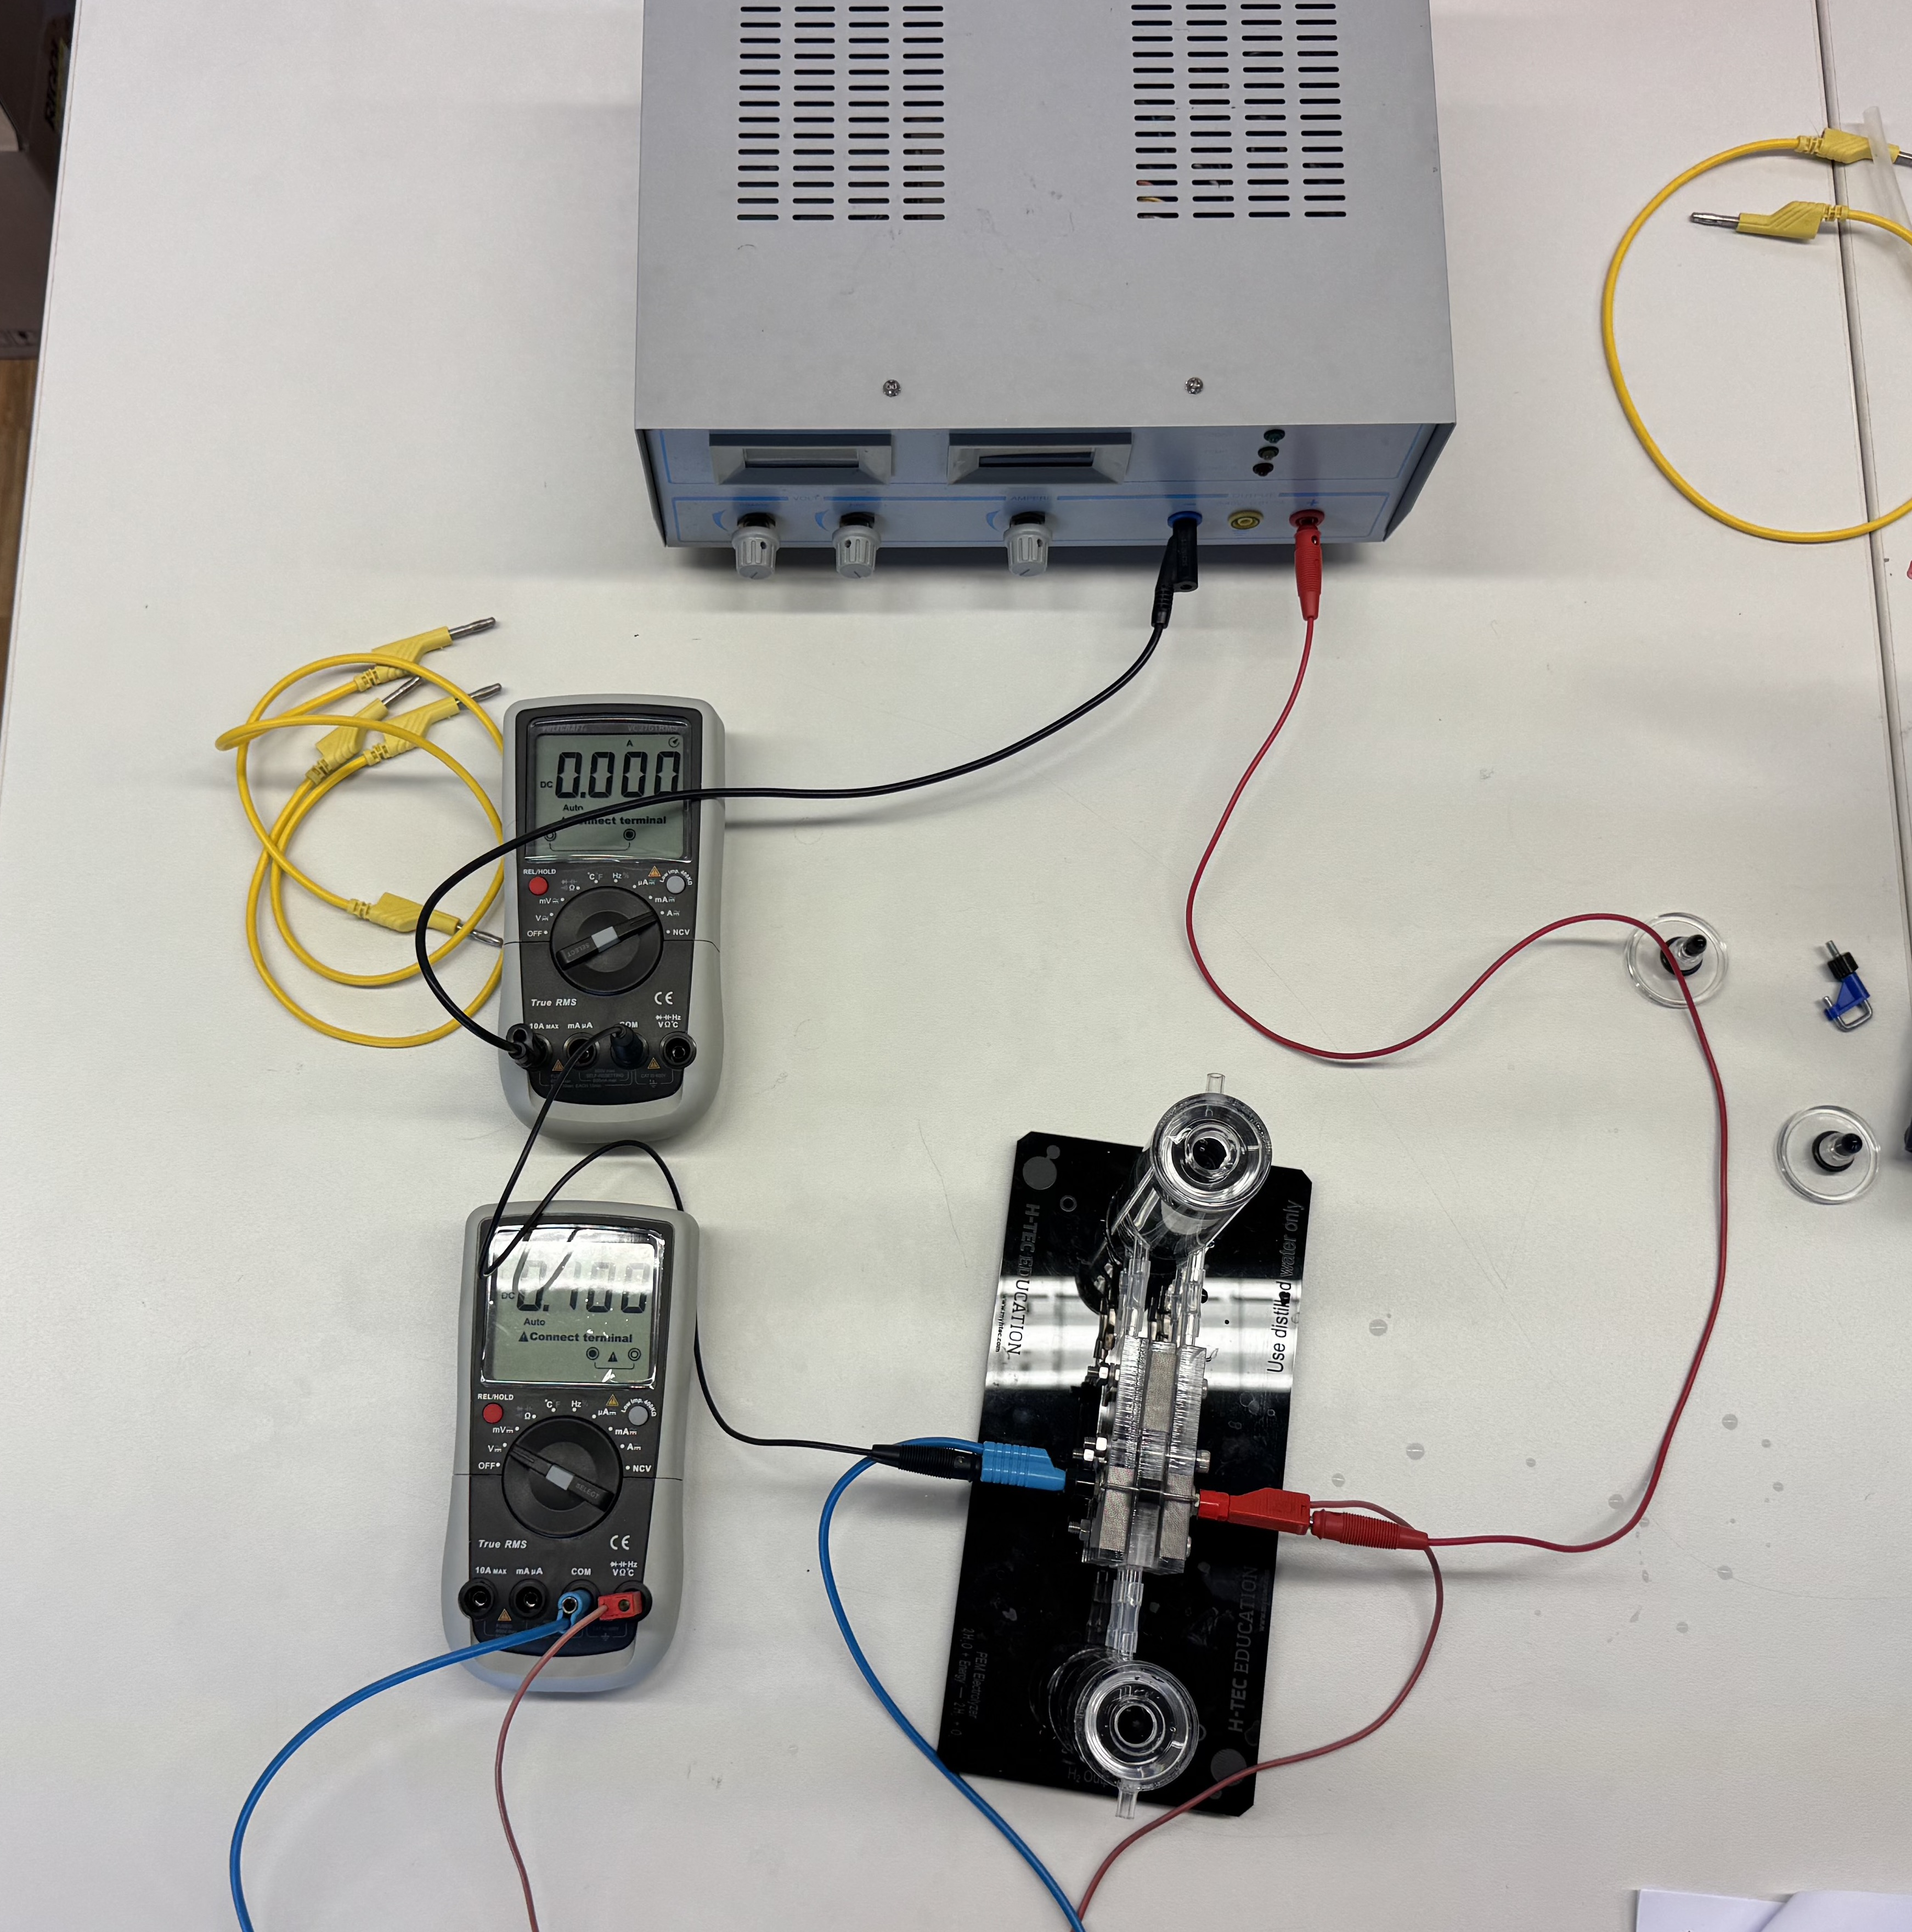
\includegraphics[width = 0.8\textwidth]{Aufbau3-2.jpeg}
	\caption{Versuchsaufbau PEM Elektrolyseur}
	\label{fig:elekt}
\end{figure}

Die beiden Vorratsbeh\"alter des Doppelzellen-Elektrolyseurs werden bis zur Markierung mit destilliertem Wasser bef\"ullt.  
Wie in Abbildung \ref{fig:elekt} zu sehen, werden Multimeter, Elektrolyseur und Netzger\"at so miteinander verbunden, dass Stromst\"arke und Spannung am Netzger\"at gemessen werden k\"onnen. Zur Bestimmung der Kennlinie wird die Spannung $U_{\text{max}}$ = 3,65 V angelegt. In regelm\"a{\ss}igen Intervallen wird die Spannung gesenkt und die Stromst\"arke gemessen. Vor jeder Aufnahme muss ca. eine Minute gewartet werden, bis sich die Prozesse innerhalb der Zelle, sowie die Werte stabilisiert haben. Auf diese Weise werden 13 U-I Wertepaare aufgenommen.
\newline
Anschlie{\ss}end wird  die Zeit gemessen, die ben\"otigt wird um 25 ml Wasserstoff herzustellen, um den Wirkungsgrad des Elektrolyseurs zu bestimmen. 
\begin{figure}[H]
	\centering
	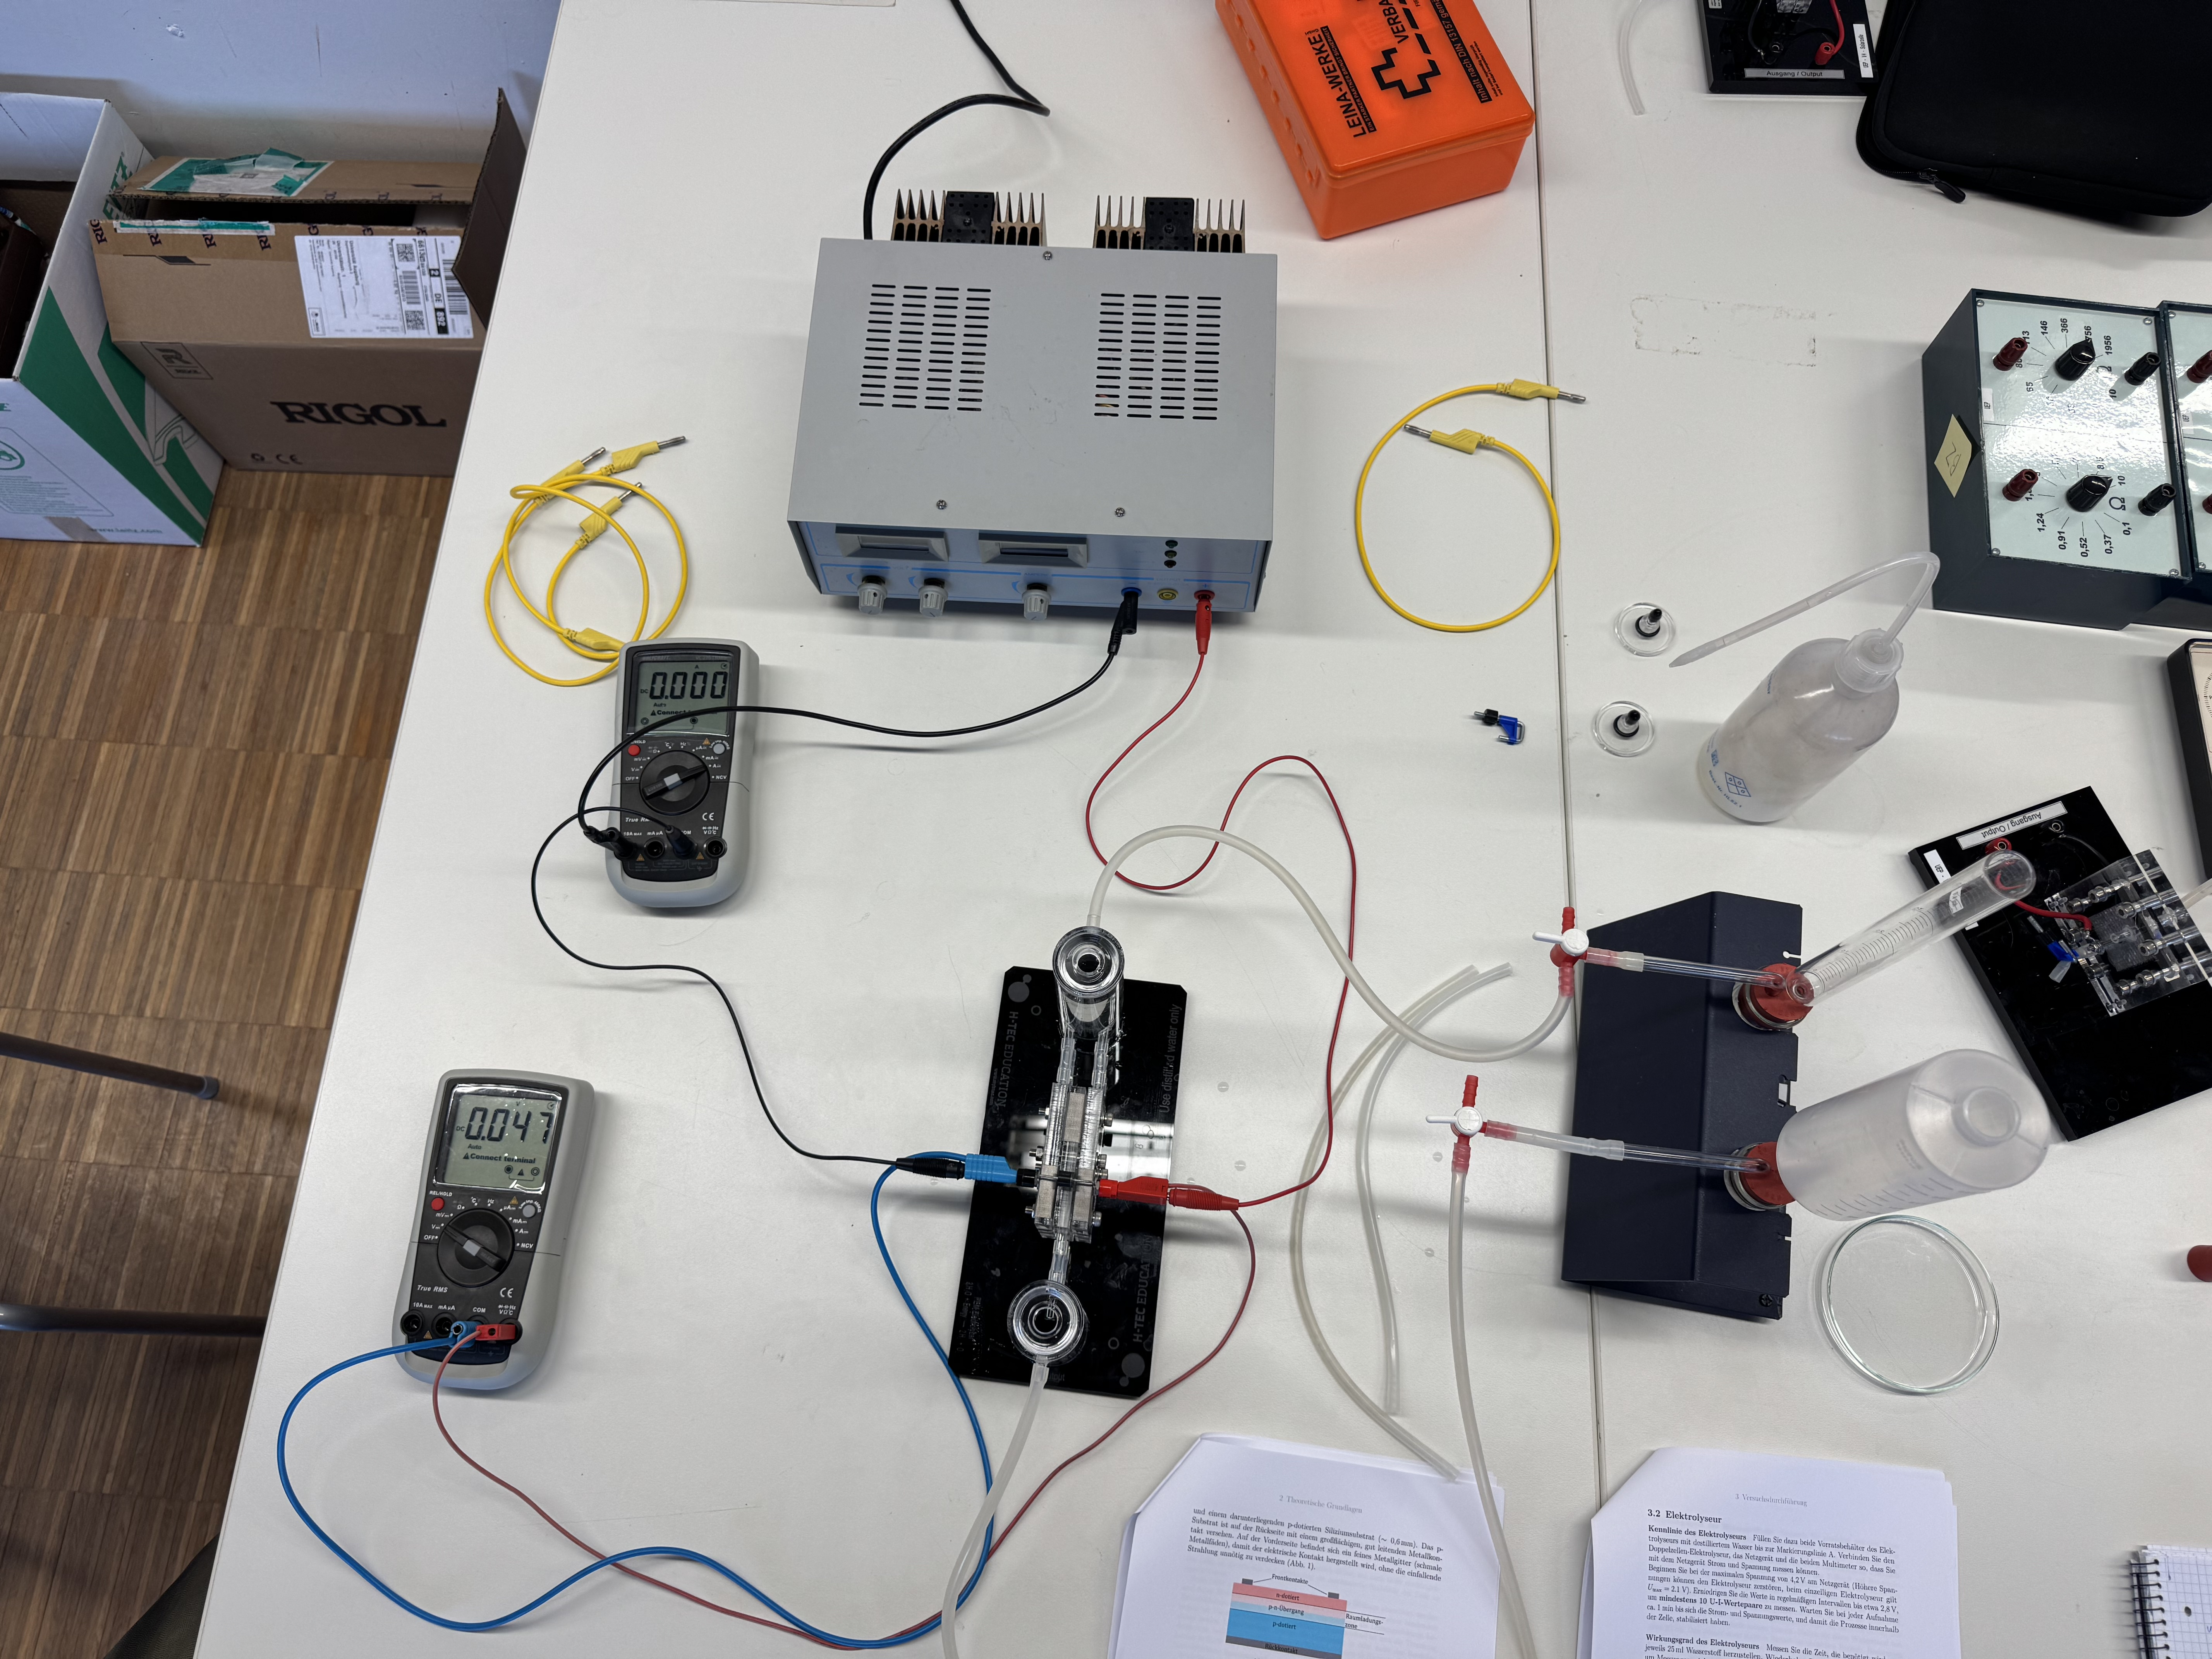
\includegraphics[width = 0.8\textwidth]{Wirkungsgrad.jpeg}
	\caption{Wirkungsgrad des Elektrolyseurs}
	\label{fig:wirk}
\end{figure}
\noindent Der Versuchsaufbau wird hierzu wie in Abbildung \ref{fig:wirk} erweitert. \"Uber zwei mit  Wasser gef\"ullten Erlenmeyerkolben werden verschlossene Messzylinder gesetzt. Die Schl\"auche der Auslassstutzen werden mit den Messzylindern \"uber ein T-Ventil verbunden. Am Netger\"at wird die Spannung $U_{\text{max}}$  angelegt. Die Zeitmessung erfolgt in drei Durchl\"aufen. Gemessen wird jeweils sobald 25ml Wasserstoff im Messzylinder vorhanden sind. Die Messungen werden bei $T_{\text{Raum}}$ = 20°C und $P_{\text{Raum}}$ = \SI{1022}{\hecto\pascal} durchgef\"uhrt.

\newpage
\subsection{Brennstoffzelle}
F\"ur den folgenden Versuchsaufbau wird der Elektrolyseurs zur st\"andigen Gasversorgung direkt an das Netzger\"at angeschlossen. Das entstehende Gas wird \"uber Schl\"auche mit einem Drei-Wege-Ventil verbunden. Hierr\"uber sind sowohl die Auffangbeh\"alter als auch die Brennstoffzelle an die Ga{\ss}produktion angeschlossen. \newline

\begin{figure}[H]
    \centering
    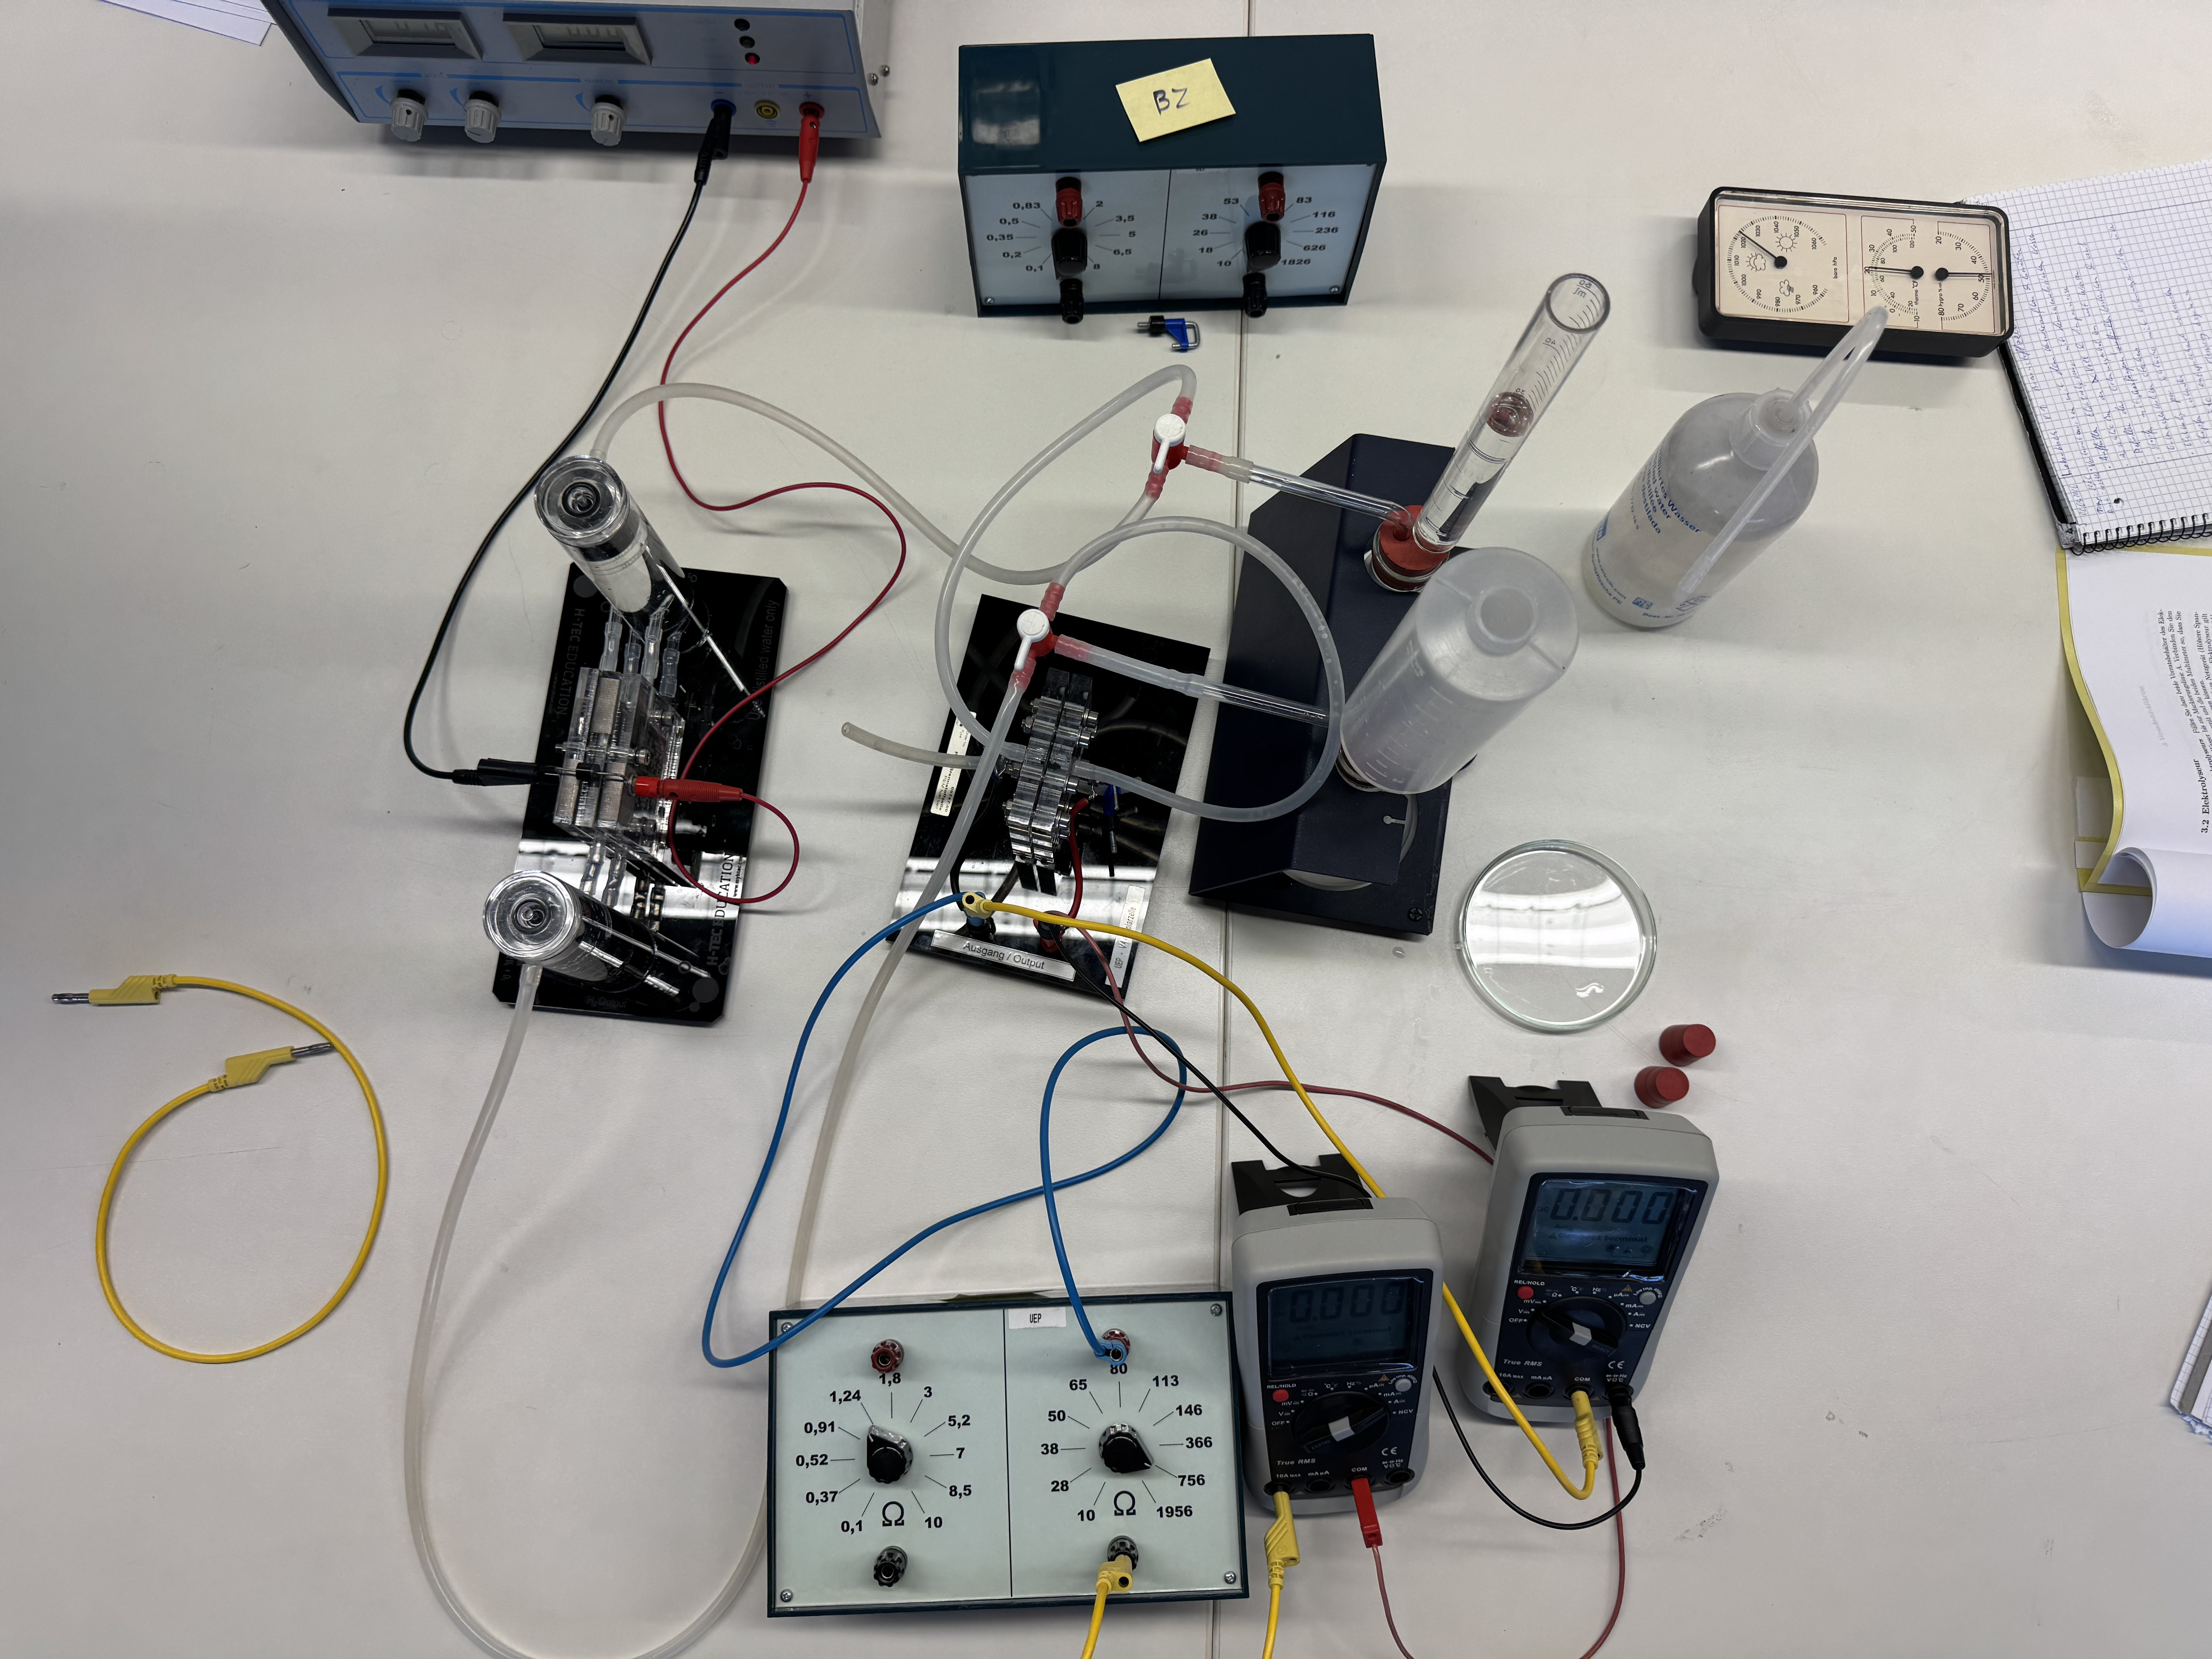
\includegraphics[width=0.8\textwidth]{Aufbau3-3.jpeg}
    \caption{Versuchsaufbau Brennstoffzelle.}
    \label{fig:brennstoffzelle}
\end{figure}

\noindent Wie in  Abbildung \ref{fig:brennstoffzelle} zu sehen ist, wird der Versuchsaufbau mit zwei Multimetern und einer Widerstandsdekade verschalten, sodass Strom und Spannung an der Brennstoffzelle gemessen gemessen werden können. Die Widerstandsdekade verf\"ugt \"uber zwei Reihen an Widerst\"anden, welche in Tabelle ~\ref{tab:widerstaende} aufgetragen sind.

\begin{table}[H]
    \centering
    \caption{Widerstandsdekaden.}
    \label{tab:widerstaende}
    \begin{tabular}{ll|ll}
        \toprule
        		\textbf{1. Dekade (Aufw\"arts)} & \textbf{R [\si{\ohm}]} &
	        \textbf{2. Dekade (Abw\"arts)} & \textbf{R [ \si{\ohm}]} \\
        		\midrule
        		$R_1$    & 10    & $R_1$    & 10   \\
        		$R_2$    & 28    & $R_2$    & 8.5  \\
	        $R_3$    & 38    & $R_3$    & 7    \\
	        $R_4$    & 50    & $R_4$    & 5.2  \\
	        $R_5$    & 65    & $R_5$    & 3    \\
	        $R_6$    & 80    & $R_6$    & 1.8  \\
	        $R_7$    & 113   & $R_7$    & 1.24 \\
	        $R_8$    & 146   & $R_8$    & 0.91 \\
	        $R_9$    & 366   & $R_9$    & 0.52 \\
	        $R_{10}$ & 756   & $R_{10}$ & 0.37 \\
	        $R_{11}$ & 1956 & $R_{11}$ & 0.1 \\
	        \bottomrule
	\end{tabular}
\end{table}

\noindent Das Netzger\"at wird auf 3,3 \si{\volt} und 2 A eingestellt, woraufhin das gesamte System f\"ur mindestens. drei Minuten mit Gas gesp\"ult wird. Um einen stabilen Zustand des Systems sicherzustellen wird vor Aufnahme der Kennlinie die Brennstoffzelle zun\"achst f\"ur f\"unf Minuten im Leerlauf und dann f\"ur weitere f\"unf Minuten mti einem Lastwiderstand von 2 \si{\ohm} betrieben.
% ---------------------------------------------------
% 4 Auswertung und Diskussion
% ---------------------------------------------------
\section{Auswertung und Diskussion}

In diesem Abschnitt werden die Messdaten ausgewertet, Unsicherheiten bestimmt und die Ergebnisse mit Literaturwerten verglichen.
\subsection{Wirkungsgrad}



% ---------------------------------------------------
% 5 Zusammenfassung
% ---------------------------------------------------
\section{Zusammenfassung}

Hier werden die wichtigsten Ergebnisse und Erkenntnisse des Versuchs kurz zusammengefasst und ein Ausblick gegeben.

% ---------------------------------------------------
% 6 Laborbuch (Anhang)
% ---------------------------------------------------
\appendix
\section{Laborbuch}

Fügen Sie hier eine gut lesbare digitale Kopie der Laborbuchseiten ein, auf denen die Messdaten dokumentiert sind.

% ---------------------------------------------------
% 7 Literaturverzeichnis
% ---------------------------------------------------
\section{Literaturverzeichnis}

\begin{thebibliography}{9}

\bibitem{Demtroeder1}
W.~Demtröder, \emph{Experimentalphysik 1: Mechanik und Wärme}, Springer, 2003.

\end{thebibliography}

\end{document}